\documentclass[conference]{IEEEtran}
\IEEEoverridecommandlockouts

%\usepackage[showframe]{geometry}% http://ctan.org/pkg/geometry

\usepackage[utf8]{inputenc}
\usepackage[lithuanian]{babel}
\usepackage[T1]{fontenc}
\renewcommand\IEEEkeywordsname{Raktažodžiai}

% The preceding line is only needed to identify funding in the first footnote. If that is unneeded, please comment it out.
\usepackage{hyperref}
\usepackage{cite}
\usepackage{amsmath,amssymb,amsfonts}
\usepackage{algorithmic}
\usepackage{graphicx}
\usepackage{textcomp}
\usepackage{xcolor}
\def\BibTeX{{\rm B\kern-.05em{\sc i\kern-.025em b}\kern-.08em
    T\kern-.1667em\lower.7ex\hbox{E}\kern-.125emX}}

\usepackage[labelsep=endash]{caption}
\renewcommand{\figurename}{pav}


\usepackage{lipsum}  


\begin{document}

\title{Orų prognozių modelių lyginamoji analizė}

\author{\IEEEauthorblockN{Liudas Kasperavičius}
\IEEEauthorblockA{\textit{Informatikos institutas} \\
\textit{Matematikos ir informatikos fakultetas}\\
Vilnius, Lietuva \\
liudas.kasperavicius@mif.stud.vu.lt}
\and
\IEEEauthorblockN{Arnas Vaicekauskas}
\IEEEauthorblockA{\textit{Informatikos institutas} \\
\textit{Matematikos ir informatikos fakultetas}\\
Vilnius, Lietuva \\
arnas.vaicekauskas@mif.stud.vu.lt}
\and
\IEEEauthorblockN{Rugilė Vasaitytė}
\IEEEauthorblockA{\textit{Informatikos institutas} \\
\textit{Matematikos ir  informatikos fakultetas}\\
Vilnius, Lietuva \\
rugile.vasaityte@mif.stud.vu.lt}
}

\maketitle

\begin{abstract}
Šiame tyrime analizuojami orų prognozių modeliai. Atlikome lyginamąją analizę naudodami iš anksto apmokytus orų prognozių modelius, tokius kaip Pangu-Weather \cite{bi2023accurate}, FourCastNet \cite{pathak2022fourcastnet}, naudojant ERA5 duomenų rinkinį \cite{data}. Gauti dviejų modelių spėjimai palyginti su tikrais duomenimis. PanguWeather modelis nuosekliai rodo žemesnes RMSE reikšmes visais žingsniais, palyginti su FourCastNet. Kodą galima peržiūrėti mūsų viešai prieinamoje \href{https://github.com/three-unicorns/time-series-forecast}{repozitorijoje}.
\end{abstract}

\begin{IEEEkeywords}
gilusis mokymasis, laiko eilutės, orų prognozės
\end{IEEEkeywords}

\section{Įvadas}

 Vidutinio laikotarpio prognozės yra svarbios siekiant priimti sprendimus įvairiose srityse, pradedant nuo atsinaujinančios energijos iki agrikultūros, tačiau jas atlikti tiksliai reikalauja daug resursų.

Prognozės dažniausiai grindžiamos skaitmeniniu orų prognozavimu (NWP), kuris prasideda nuo apibrėžtų fizikos lygčių, vėliau paverstų į kompiuterinius algoritmus, vykdomus superkompiuteriuose. Tačiau lygčių ir algoritmų kūrimas užima daug laiko ir reikalauja gilių žinių, taip pat brangių skaičiavimo išteklių, kad būtų galima tiksliai prognozuoti.

Gilusis mokymasis siūlo kitokį metodą: vietoj fizinių lygčių naudojami duomenys orų prognozavimo sistemai sukurti. Tokie modeliai siūlo mažesnes skaičiavimo sąnaudas, palyginti su NWP modeliais \cite{schultz2021}. Pangu-Weather \cite{bi2023accurate} ir FourCastNet  (Fourier ForeCasting Neural Network) \cite{pathak2022fourcastnet} yra apmokyti dešimtmečiais istorinių orų duomenimimis, kad modelis prognozuotų orų raidą. 

\section{Metodai}


\subsection{FourCastNet modelio architektūros apžvalga}

FourCastNet modelio architektūros pagrindą sudaro regėjimo transformatoriai, kurie praktiniuose taikymuose gali pakeisti konvoliucinius neuroninius tinklus (CNNs) dėl savo gebėjimo išgauti gerus rezultatus naudojant reliatyviai nedidelius skaičiavimams skirtus išteklius \cite{dosovitskiy2020image}. Orų prognozės problema reikalauja didelės rezoliucijos įvesties duomenų ir rezultatų norint, kad jie būtų naudingi praktikoje. Tai yra problema, nes regėjimo transformatorių principas yra žetonų maišymo algoritmas, kuris turi kvadratinę priklausomybę nuo įvesties pikselių skaičiaus \cite{guibas2021adaptive}. Dėl šios priežasties FourCastNet architektūra yra patobulinta naudojant Furjė Neuroninų Operatorių (FNO) mokymosi principu, kuris išsprendžia žetonų maišymo problemą ir padaro algoritmą nepriklausomą nuo įvesties duomenų rezoliucijos \cite{guibas2021adaptive}. Ši architektūra yra viena iš pirmųjų, kuri savo laiku pasiūlė praktikoje pritaikomą alternatyvą, galinčią konkuruoti su skaitmeninių orų prognozavimų sistemoms dėl savo greičio ir mažų energijos sąnaudų, bet ne dėl tikslesnių rezultatų  \cite{pathak2022fourcastnet}.

\begin{figure}[htb!] % puslapio viršuje
\centerline{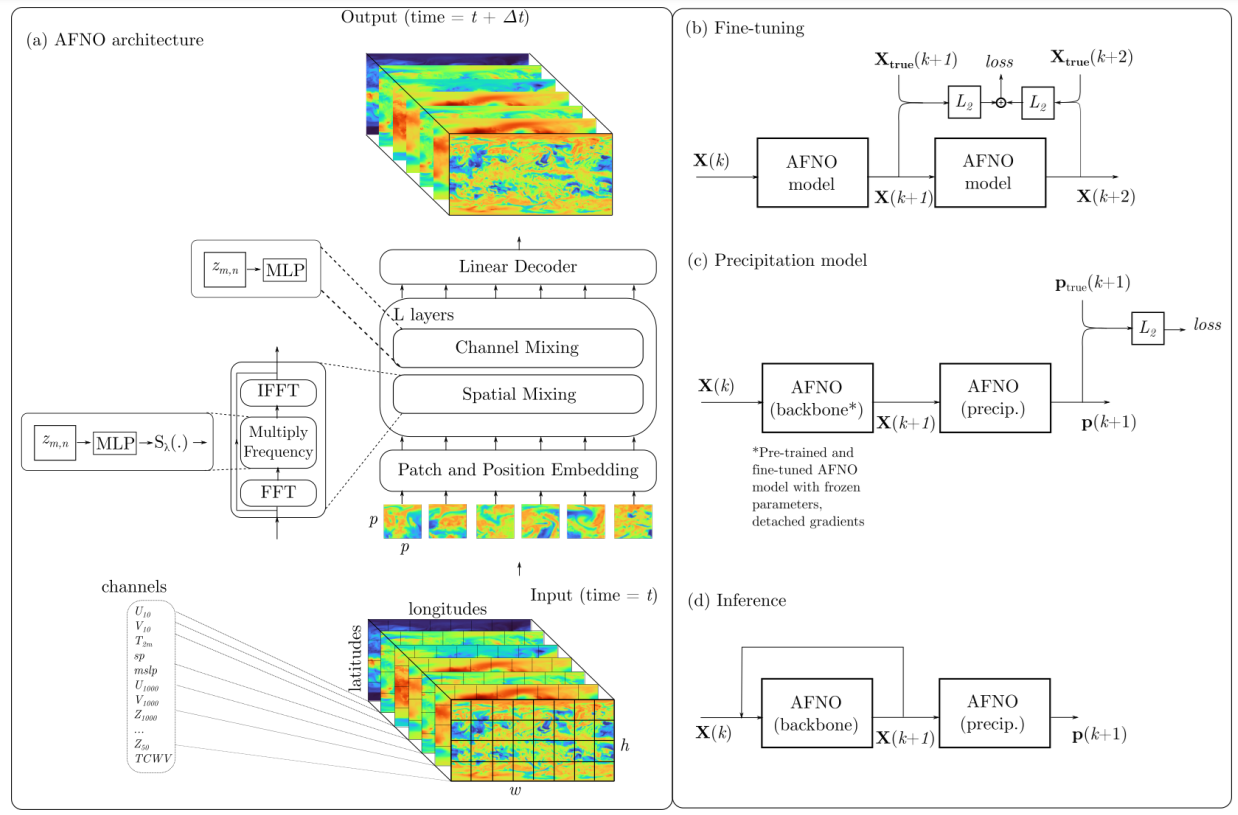
\includegraphics[width=0.5\textwidth]{img/fourcastnet-architecture.png}}
\caption{FourCastNet architektūra}
\label{fig1}
\end{figure}

\subsection{Pangu-weather modelio architektūros apžvalga}

Pangu-weather modelio architektūrą sudaro enkoderio ir dekoderio pora kartu su lopinėlių įstatymo (patch embedding) ir atgavimo (patch recovery) sluoksniais \cite{bi2022pangu}. Lopinėlių įstatymo sluoksnis sumažina įvesties duomenų dydį prieš paduodant juos tolimesniems sluoksniams. Enkoderis ir dekoderis yra simetriški ir turi po 8 sluoksnius. Pirmi du enkoderio sluoksniai nekeičia įvesties dimensijų, tačiau padidina įvesties duomenų kanalų skaičių. Tolimesni 6 enkoderio sluoksniai mažina įvesties dimensiją naudojant Swin tranformerius, kurie leidžia efektyviau atlikti dėmesio skaičiavimus (self-attention) padalinant įvesties duomenis į nepersidengiančius langus \cite{liu2021swin}. Dekoderis analogiškai atlieka įvesties duomenų padidinimą (upsampling). Architektūroje taip pat numatyta antro enkoderio sluoksnio ir septinto dekoderio sluoksnio jungtis (concatination) ties kanalų dimensija. 

\begin{figure}[htb!] % puslapio viršuje
\centerline{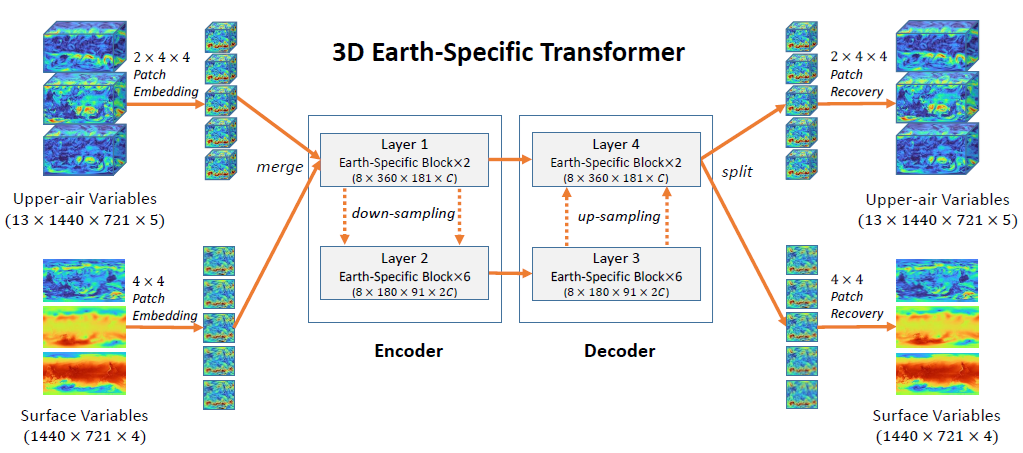
\includegraphics[width=0.5\textwidth]{img/pangu-weather-architecture.png}}
\caption{Pangu-Weather architektūra}
\label{fig1}
\end{figure}

\newpage
\subsection{Nuostolių funkcija}

Šaknies vidurkio kvadrato paklaida (RMSE) randama pagal formulę:

\begin{equation}
\mathcal{L} = \sqrt{\frac{1}{n} \sum_{i=1}^n (y_i - \hat{y}_i)^2}
\label{eq:lygtis1}
\end{equation}

Ši formulė apskaičiuoja prognozių klaidų  standartinį nuokrypį, matuojant, kiek prognozuojamos vertės skiriasi nuo faktinių verčių.

% Pristatote naudojamus metodus

% \begin{equation}
% \mathcal{L}({\bf X}, {\bf Y}) = \frac{1}{w \cdot h} \sum_{i=1}^h \sum_{j=1}^w (X_{i, j} - Y_{i, j})^2
% \label{eq:lygtis1}
% \end{equation}

% Taikyta nuostolių funkcija ~\eqref{eq:lygtis1}.

% \begin{align}
% y & = f(x) \nonumber \\
% f & = f_1(f_2(x))
% \label{eq:lygtis2}
% \end{align}

% Taikytas modelis ~\eqref{eq:lygtis2}.


\section{Duomenys}

\subsection{Duomenų rinkinys}
Modeliui testuoti buvo naudojamas „ERA5 hourly data on single levels from 1940 to present“ duomenų rinkinys iš Copernicus Climate Data Store (CDS). CDS suteikia vieną prieigos tašką prie kokybiškų klimato duomenų rinkinių, gautus iš Žemės stebėjimų. Prieiga prie duomenų yra atvira, nemokama ir neribota. 

Naudojamas duomenų rinkinys ERA5 \cite{data} laikomas vienu geriausiu žinomu rinkiniu vertinti daugumą atmosferos kintamųjų \cite{evaluationoftheERA5}. ERA5 yra penktosios kartos ECMWF reanalizė, duomenys prieinami nuo 1940 metų, suteikiamas globalinis padengimas. 

\subsection{Duomenų formatas}
Duomenys išsaugoti GRIB (GRIdded Binary or General Regularly-distributed Information in Binary form). GRIB yra glaustas duomenų formatas, dažnai naudojamas meteorologijoje istoriniams ir prognoziniams orų duomenims saugoti. Kiekvienas GRIB įrašas turi dvi dalis - dalį, kuri apibūdina įrašą, tai yra antraštė, ir pačius dvejetainius duomenis. Duomenimis manipuliuoti buvo naudojama cfgrib Python biblioteka, sukurta skaityti ir rašyti GRIB failus naudojant xarray biblioteką.   

\subsection{Testuojami duomenys}
Pangu-Weather \cite{bi2023accurate} ir FourCastNet \cite{pathak2022fourcastnet} buvo testuojami nuo 0-inės laiko eilutės 2024-05-01T12:00:00, 5 laiko eilutes į priekį kas 6 valandas. Lyginami duomenys apėmė Šiaurės Rytų Europos regioną, tyrime vaizduojami šie parametrai:
\begin{enumerate}
\item 2 metrų aukštyje nustatyta temperatūra, K. Šis parametras nurodo oro temperatūrą dviem metrais virš žemės, vandens arba vidaus vandenų paviršiaus.
\item 10 metrų aukštyje nustatytos vėjo U komponentės (rytinė kryptis), m/s. Šis parametras nurodo oro srauto greitį, judant į rytus, esant dešimties metrų aukštyje nuo Žemės paviršiaus.
\item 10 metrų aukštyje nustatytos vėjo V komponentės (šiaurinė kryptis), m/s. Šis parametras apibūdina oro srauto greitį, judant į šiaurę, esant dešimties metrų aukštyje nuo Žemės paviršiaus. 
\end{enumerate}
Šie duomenys padeda suprasti horizontalaus 10 metrų aukščio vėjo greitį ir kryptį, sujungus U ir V vėjo komponentes.

% \begin{figure}[!h] % įterpti čia
% \centerline{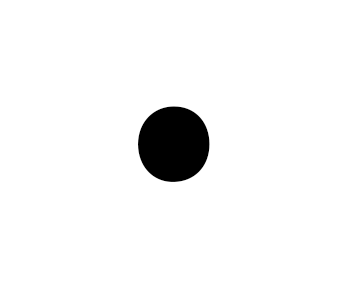
\includegraphics{fig1.png}}
% \caption{Paveikslėlio aprašas.}
% \label{fig}
% \end{figure}

\section{Rezultatai}

~\ref{fig1} pav. pavaizduota 0-inės laiko eilutės 2024-05-01T12:00:00 parametrai Šiaurės-Rytų Žemės dalyje. Tai įvesties duomenys naudojami abiems modeliams testuoti. Pagal juos modeliai atliko prognozes 5 laiko eilutes į priekį. 

\begin{figure}[htb!] % puslapio viršuje
\centerline{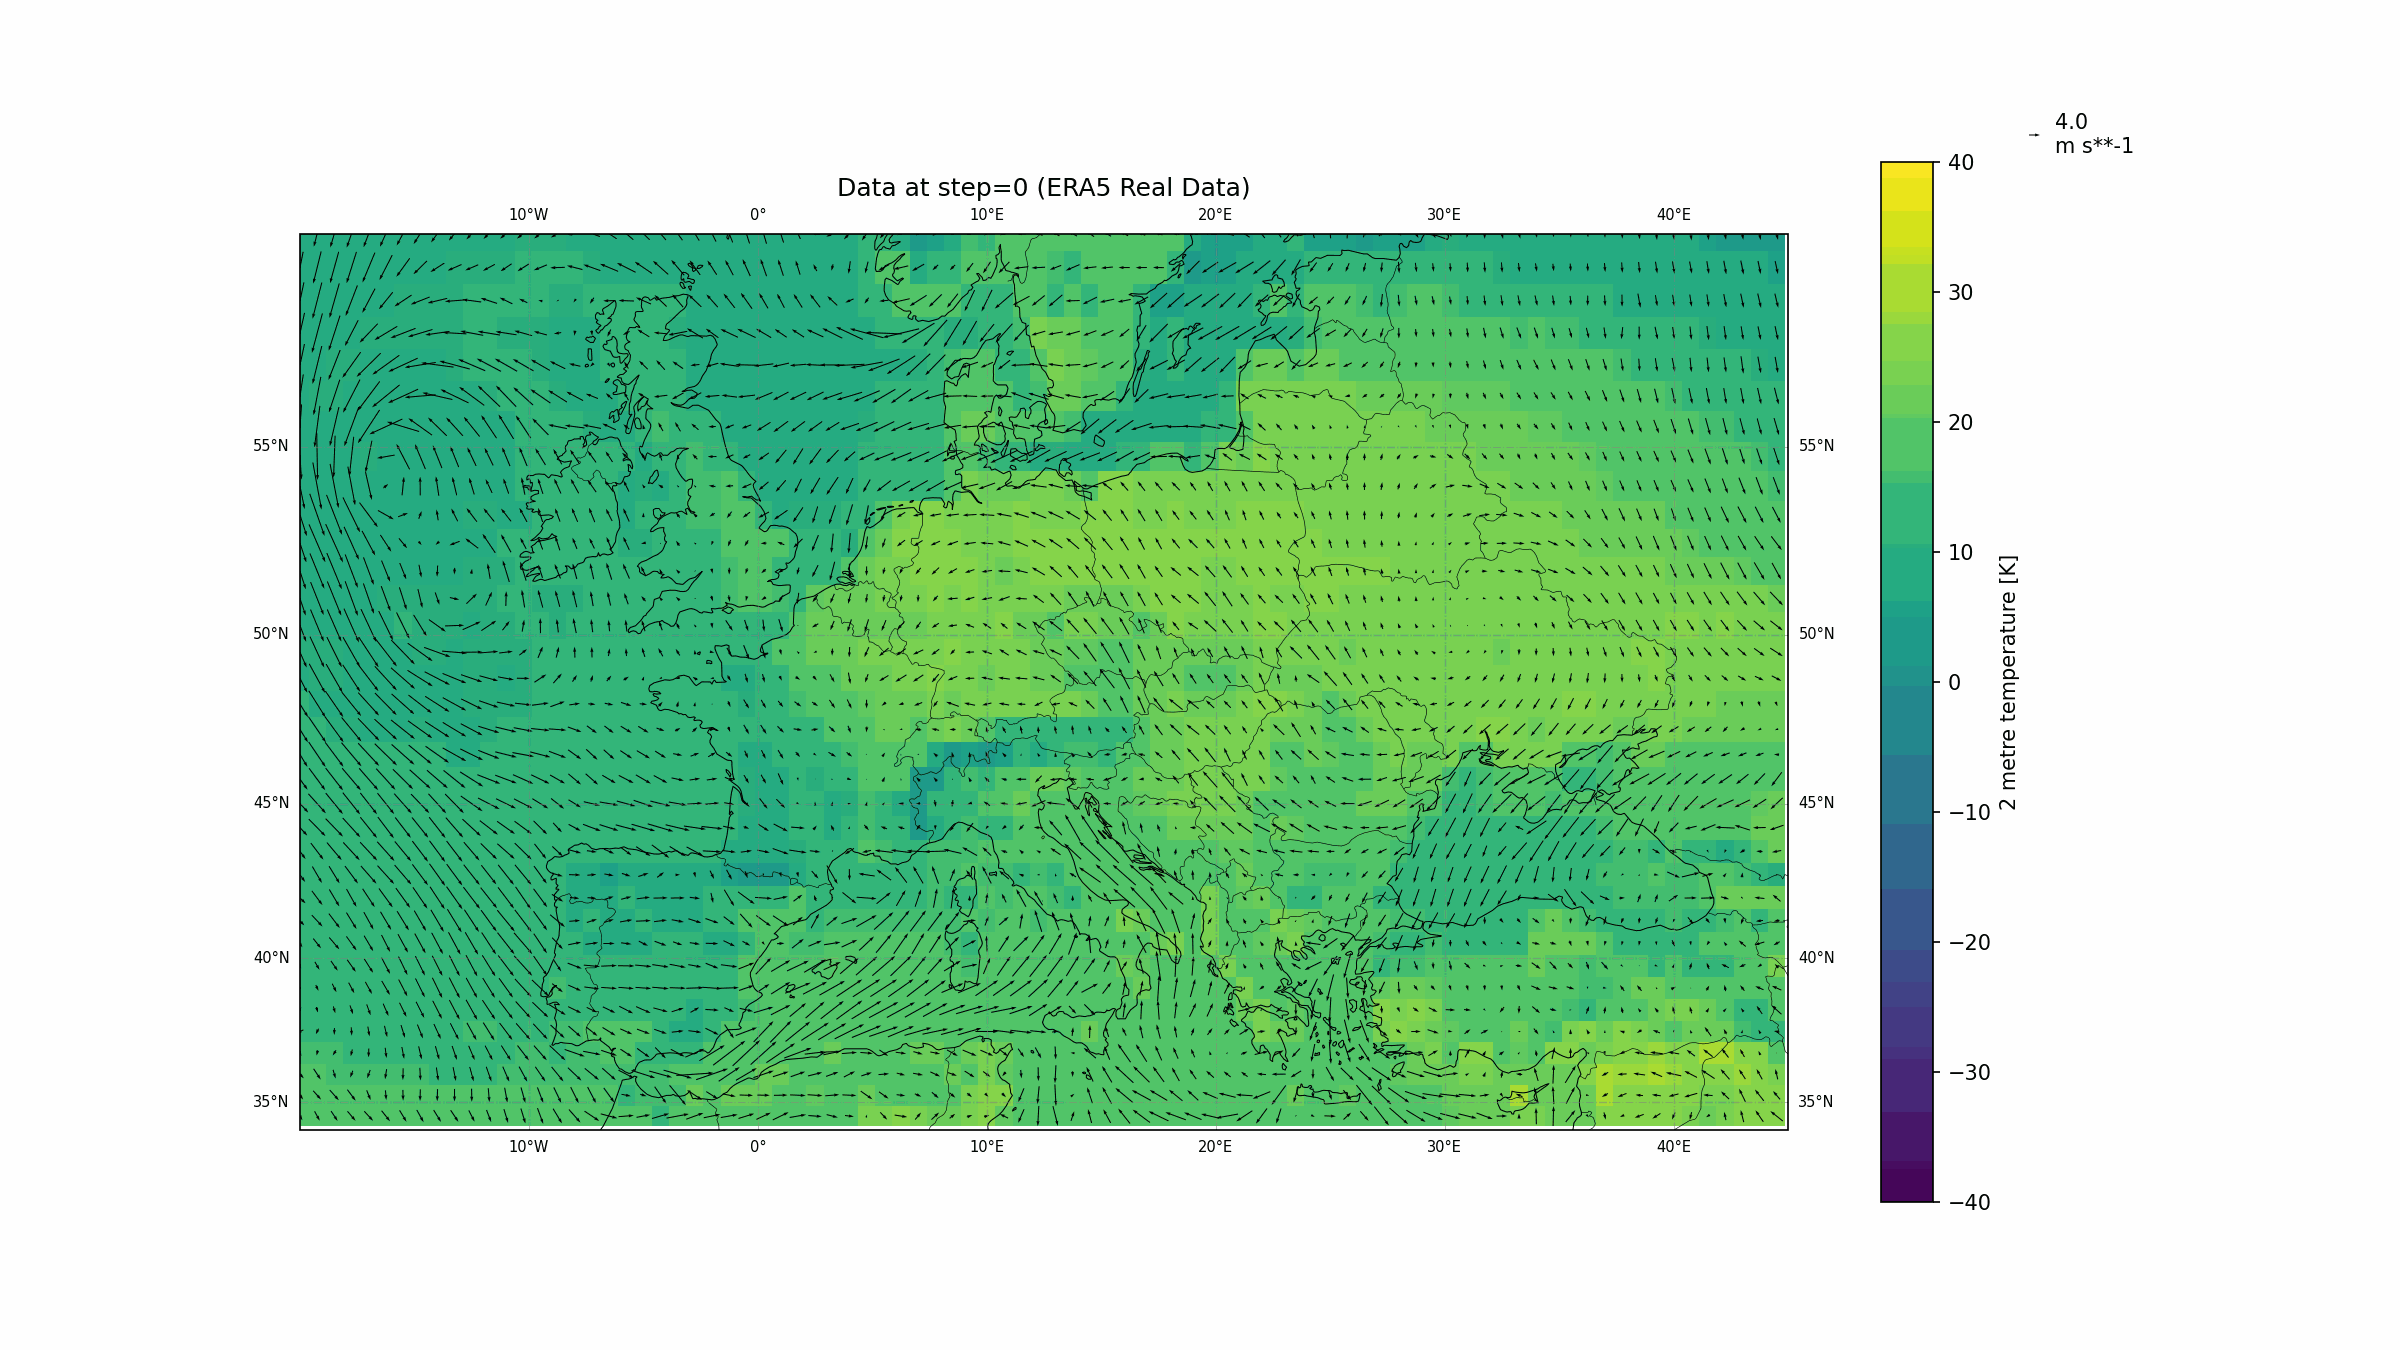
\includegraphics[width=0.53\textwidth]{img/frame_0_delay-1s.png}}
\caption{Įvesties duomenys. Tikra vėjo kryptis, greitis ir temperatūra 2024-05-01T12:00:00}
\label{fig1}
\end{figure}

~\ref{fig5} pav., ~\ref{fig6} pav., ~\ref{fig7} pav., ~\ref{fig8} pav., ~\ref{fig9} pav. matomi realūs duomenys, FourCastNet ir PanguWeather prognozė.

~\ref{fig10} pav., ~\ref{fig11} pav., ~\ref{fig12} pav., ~\ref{fig13} pav., ~\ref{fig14} pav. matomi skirtumai tarp realių duomenų ir modelių prognozių.

~\ref{fig4} pav. apskaičiuotas RMSE tarp realių duomenų ir modelių prognozių. 
\begin{figure}[htb!] % puslapio viršuje
\centerline{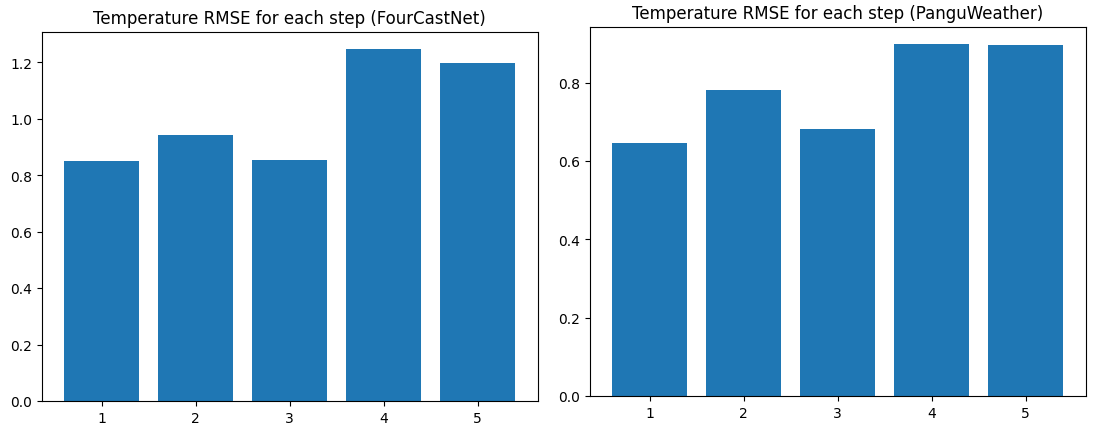
\includegraphics[width=0.5\textwidth]{img/RMSE.png}}
\caption{Temperatūros RMSE}
\label{fig4}
\end{figure}

PanguWeather nuosekliai parodo žemesnes RMSE reikšmes visais žingsniais, lyginant su FourCastNet. Tai leidžia manyti, kad PanguWeather yra tikslesnis prognozuojant temperatūrą modelis. Žemesnės RMSE reikšmės PanguWeather rodo, kad jis gali būti patikimesnis tokioms užduotims, kur reikalinga tiksli temperatūros prognozė. Visgi prognozę atlikti su PanguWeather užtruko 10 kartų ilgiau nei su FourCastNet 

\begin{figure*}[!t]
\centerline{\includegraphics[width=0.85\textwidth]{img/step1.png}}
\caption{Vėjo kryptis, greitis ir temperatūra 2024-05-01T18:00:00}
\label{fig5}
\end{figure*}

\begin{figure*}[htb!] % puslapio viršuje
\centerline{\includegraphics[width=0.85\textwidth]{img/step2.png}}
\caption{Vėjo kryptis, greitis ir temperatūra 2024-05-02T00:00:00}
\label{fig6}
\end{figure*}

\begin{figure*}[htb!] % puslapio viršuje
\centerline{\includegraphics[width=0.85\textwidth]{img/step3.png}}
\caption{Vėjo kryptis, greitis ir temperatūra 2024-05-02T12:00:00}
\label{fig7}
\end{figure*}

\begin{figure*}[htb!] % puslapio viršuje
\centerline{\includegraphics[width=0.85\textwidth]{img/step4.png}}
\caption{Vėjo kryptis, greitis ir temperatūra 2024-05-02T18:00:00}
\label{fig8}
\end{figure*}

\begin{figure*}[htb!] % puslapio viršuje
\centerline{\includegraphics[width=0.85\textwidth]{img/step5.png}}
\caption{Vėjo kryptis, greitis ir temperatūra 2024-05-03T00:00:00}
\label{fig9}
\end{figure*}
% %\lipsum[2-10]


\begin{figure*}[htb!] % puslapio viršuje
\centerline{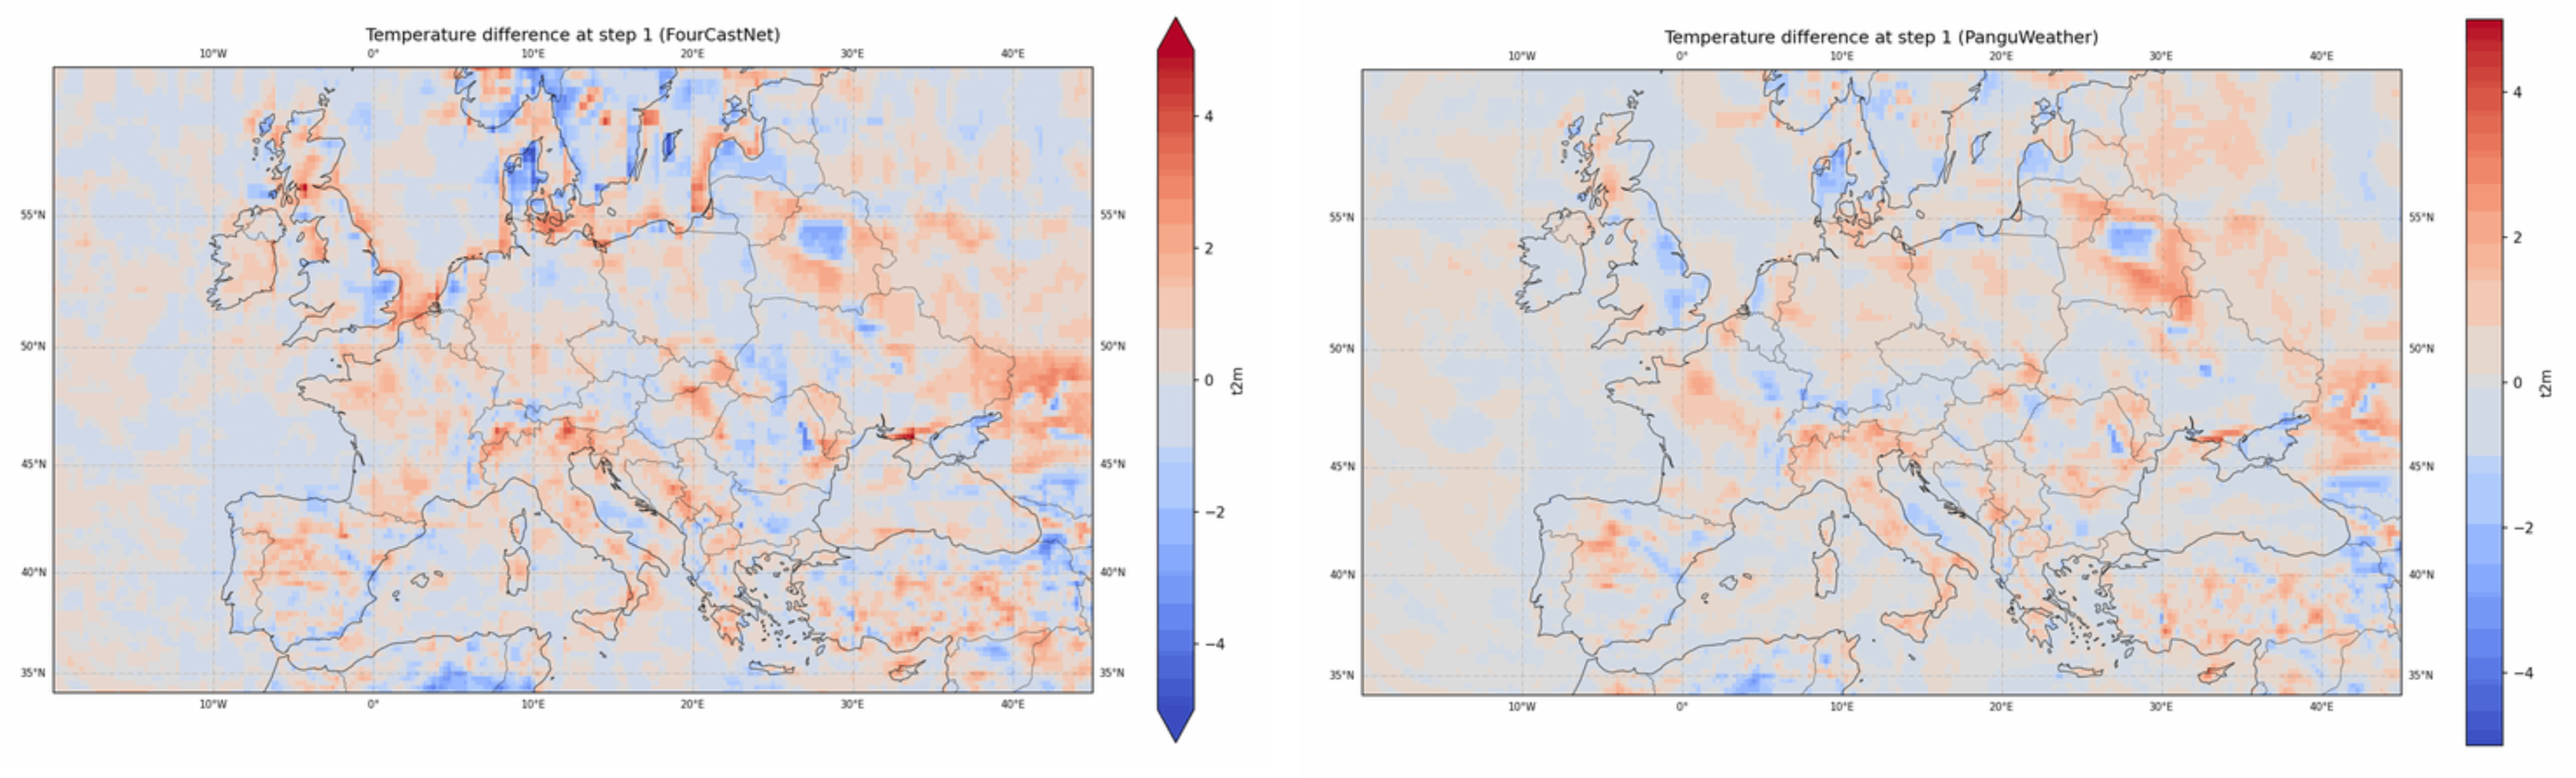
\includegraphics[width=\textwidth]{img/diffstep1.png}}
\caption{Skirtumas tarp modelių prognozių ir realių duomenų (FourCastNet ir PanguWeather)}
\label{fig10}
\end{figure*}

\begin{figure*}[htb!] % puslapio viršuje
\centerline{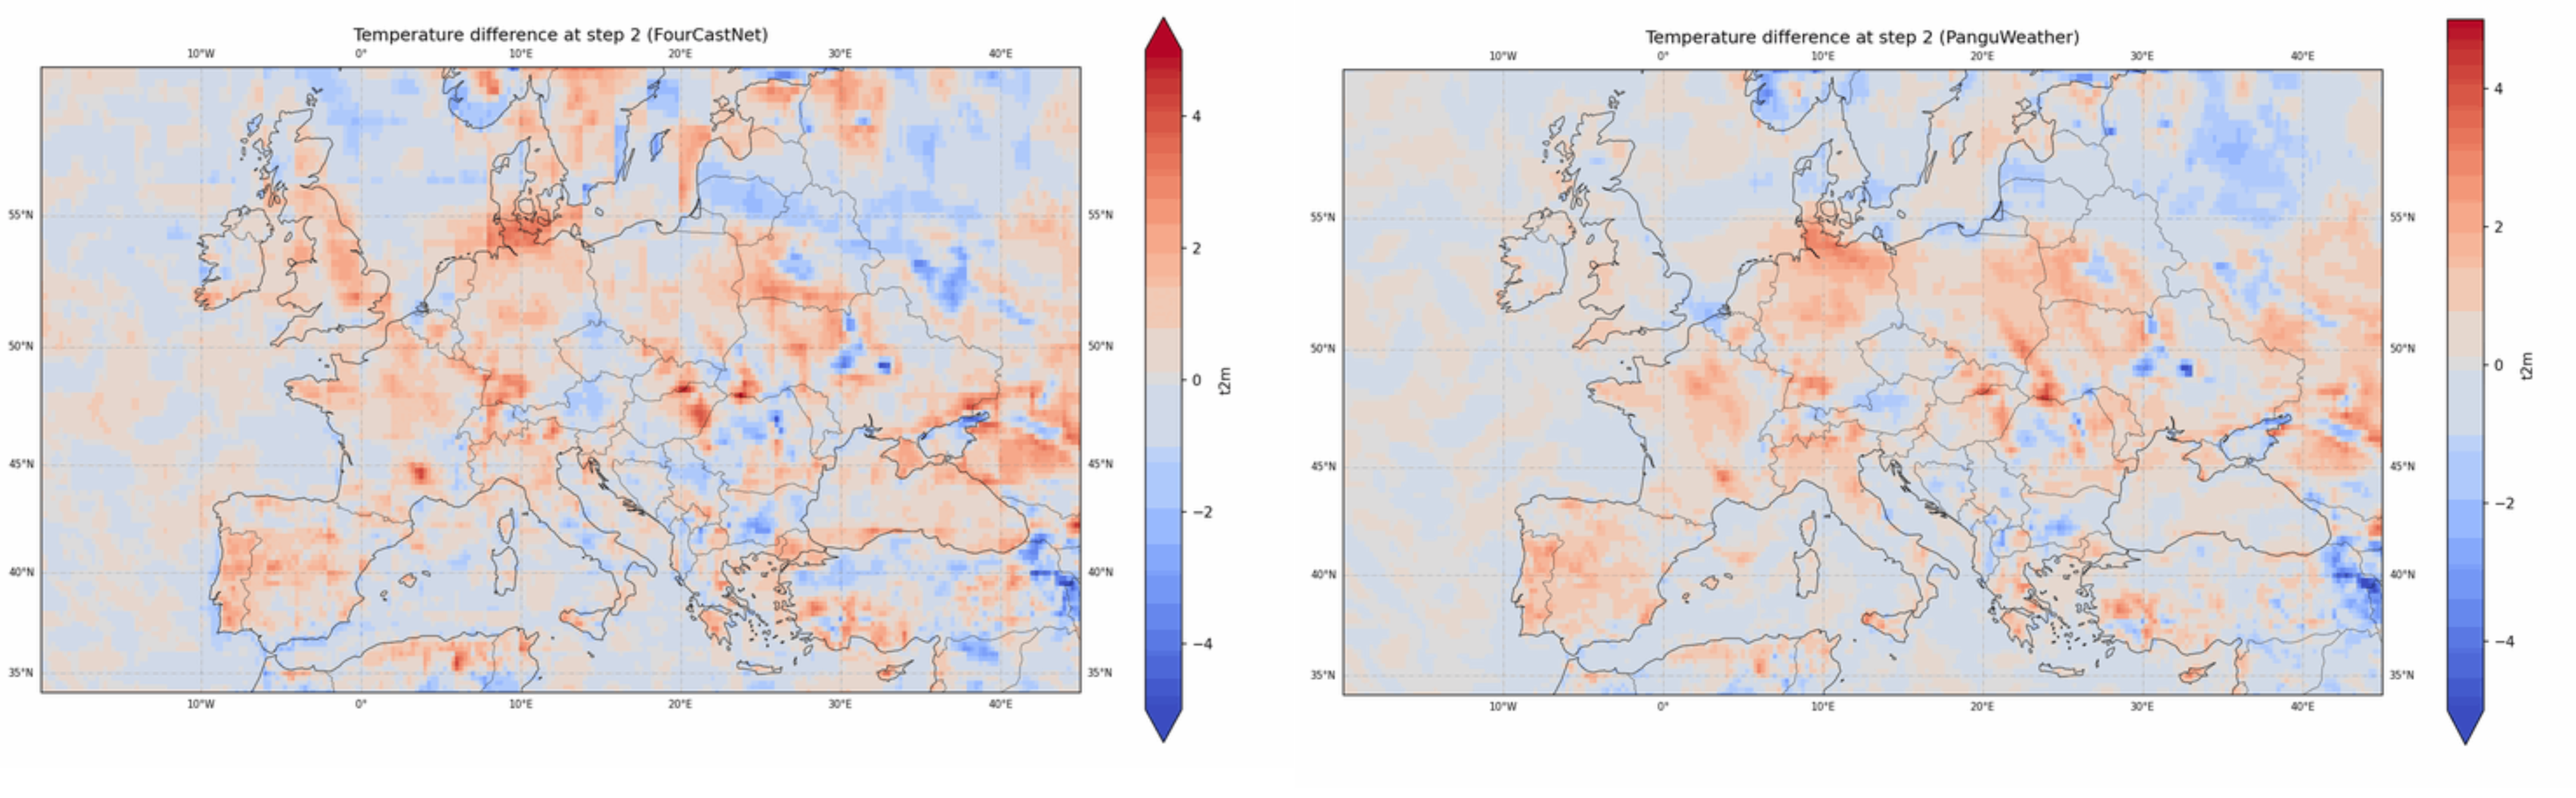
\includegraphics[width=\textwidth]{img/diffstep2.png}}
\caption{Skirtumas tarp modelių prognozių ir realių duomenų (FourCastNet ir PanguWeather)}
\label{fig11}
\end{figure*}


\begin{figure*}[htb!] % puslapio viršuje
\centerline{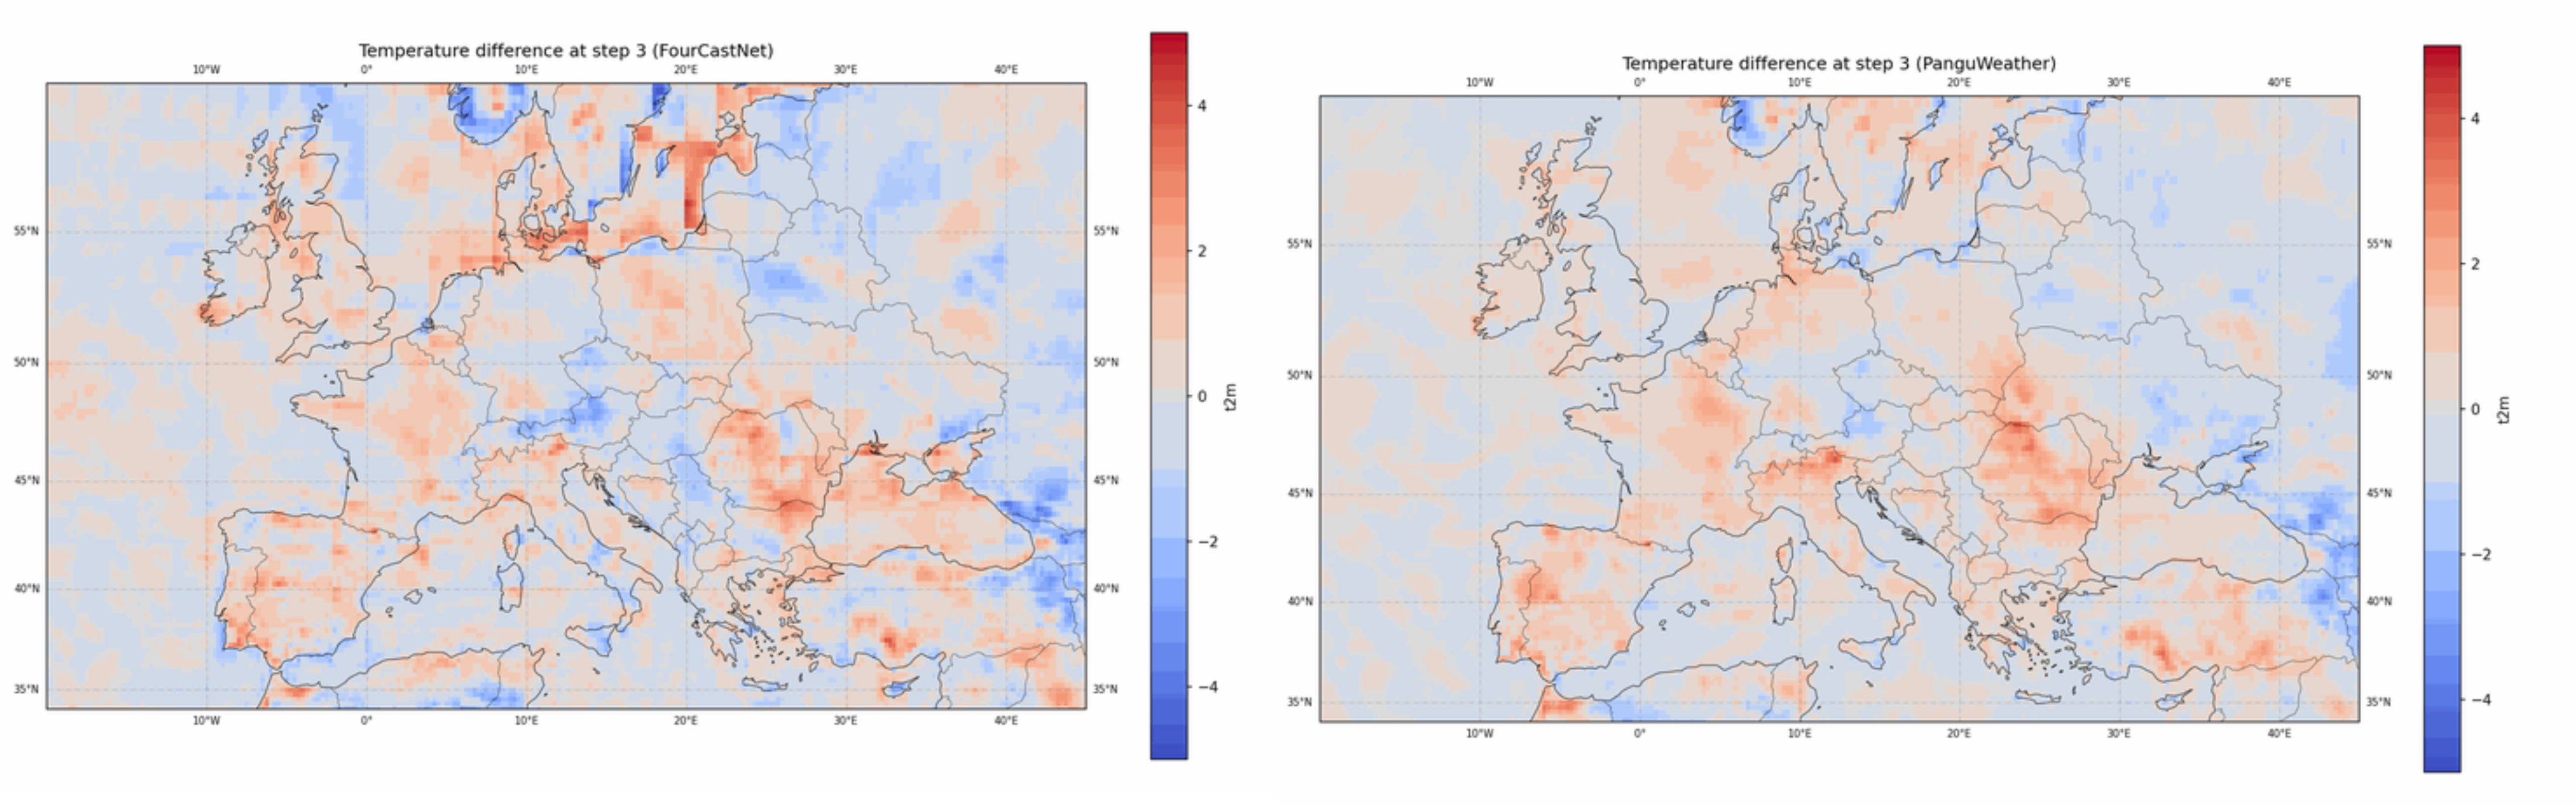
\includegraphics[width=\textwidth]{img/diffstep3.png}}
\caption{Skirtumas tarp modelių prognozių ir realių duomenų (FourCastNet ir PanguWeather) 2024-05-02T12:00:00}
\label{fig12}
\end{figure*}


\begin{figure*}[htb!] % puslapio viršuje
\centerline{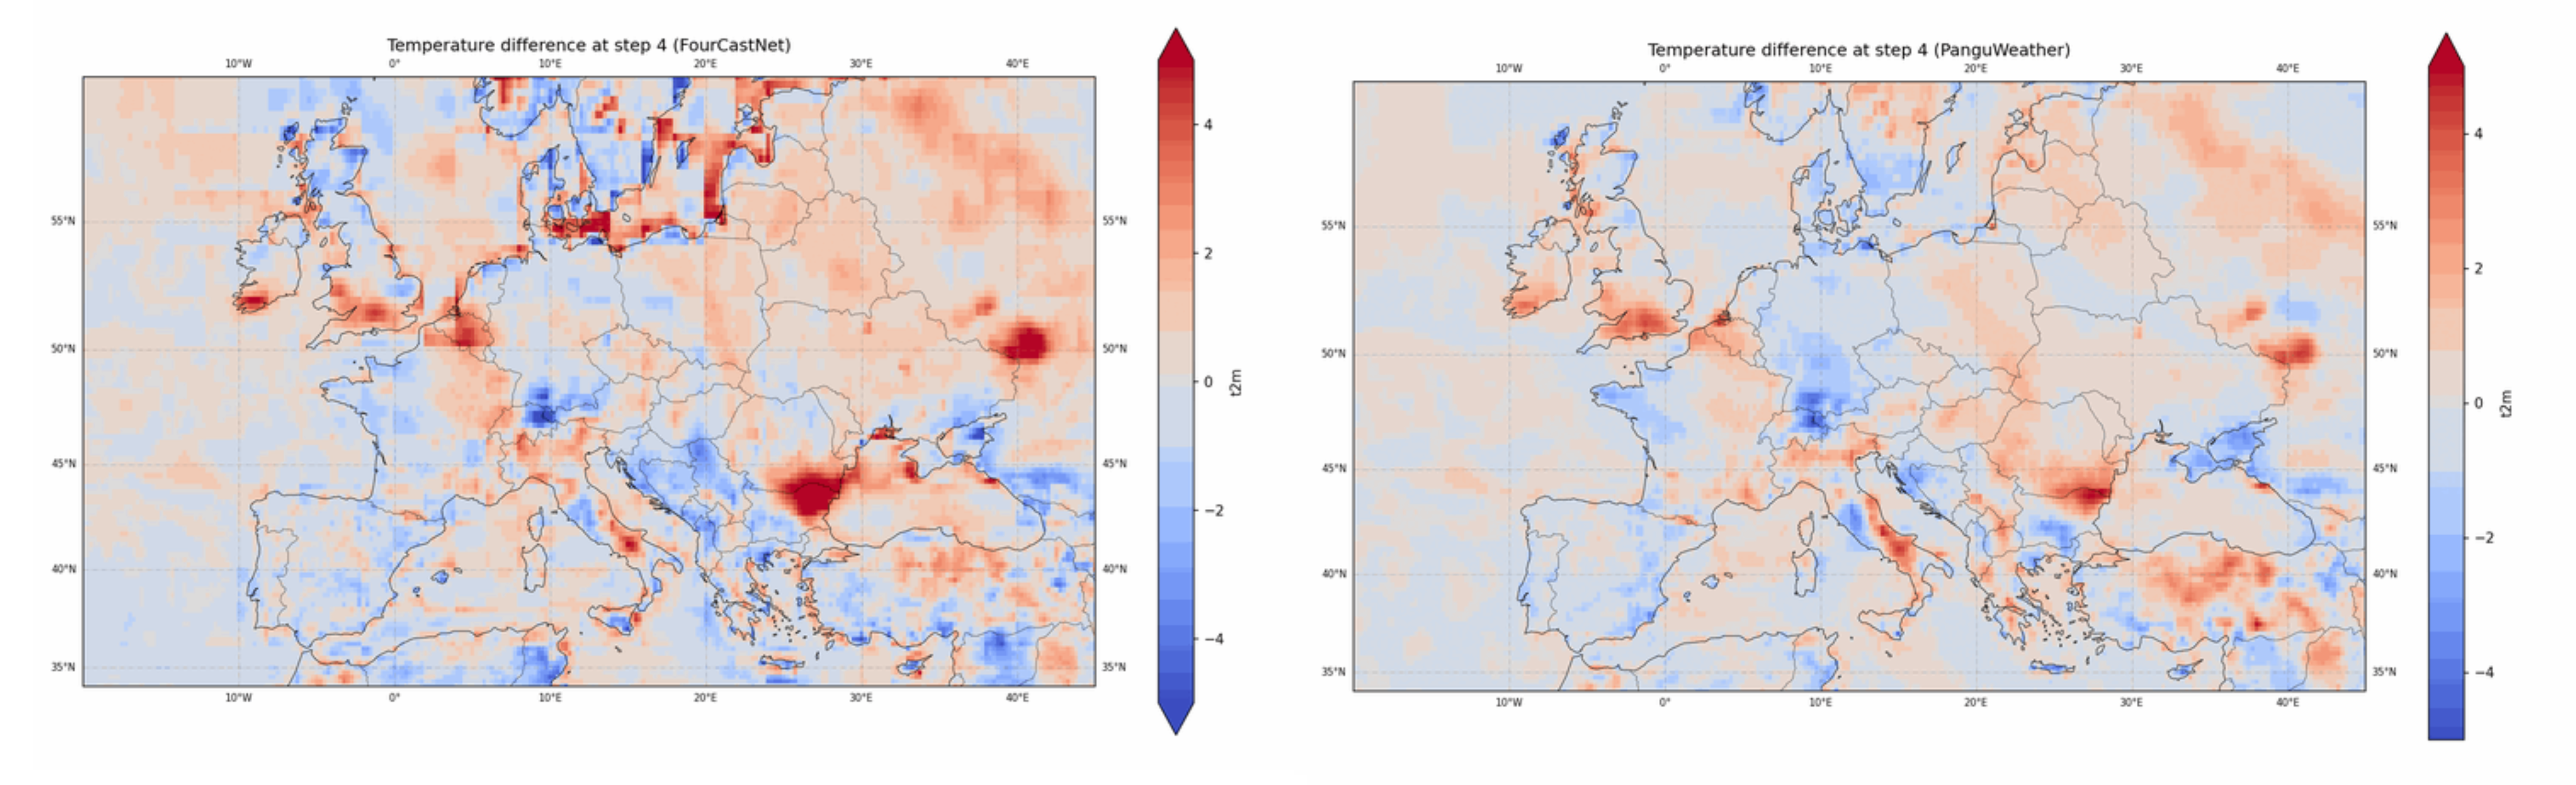
\includegraphics[width=\textwidth]{img/diffstep4.png}}
\caption{Skirtumas tarp modelių prognozių ir realių duomenų (FourCastNet ir PanguWeather) 2024-05-02T18:00:00}
\label{fig13}
\end{figure*}

\begin{figure*}[htb!] % puslapio viršuje
\centerline{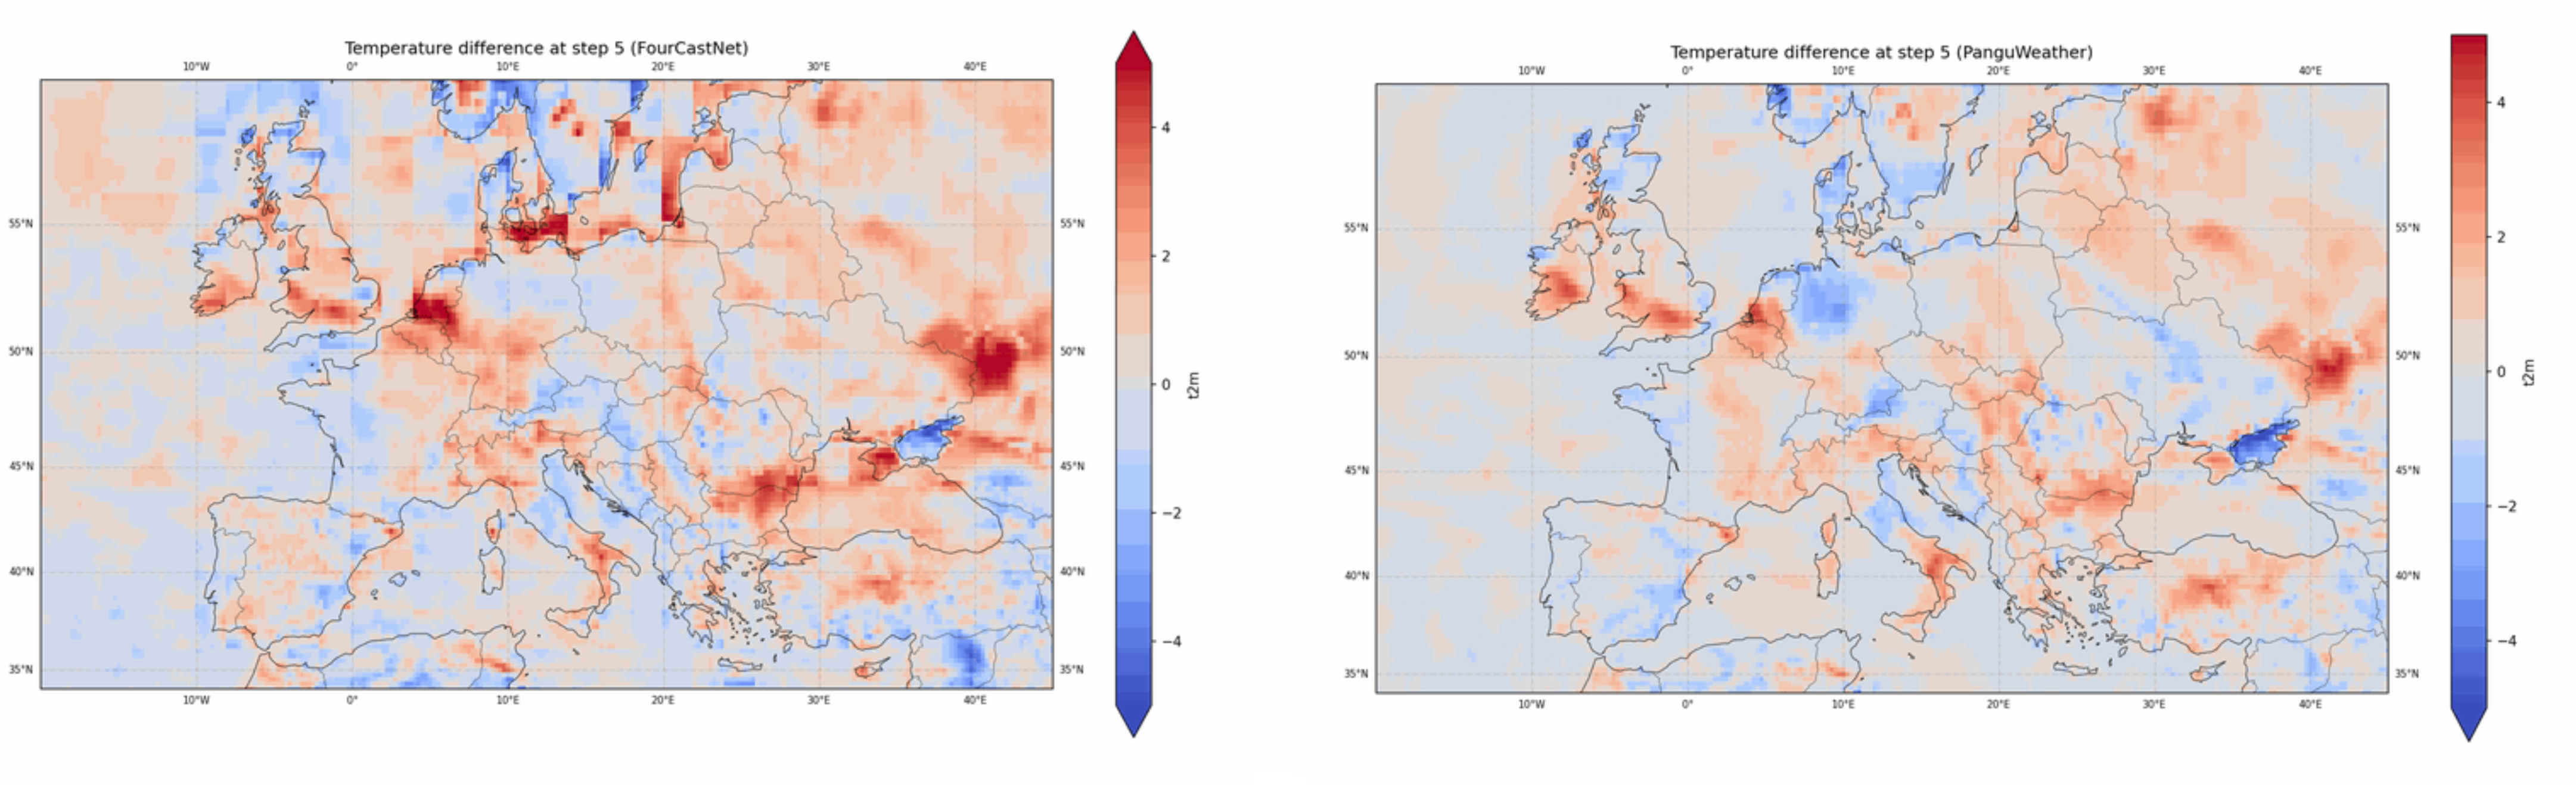
\includegraphics[width=\textwidth]{img/diffstep5.png}}
\caption{Skirtumas tarp modelių prognozių ir realių duomenų (FourCastNet ir PanguWeather) 2024-05-03T00:00:00}
\label{fig14}
\end{figure*}

\bibliographystyle{plain}
\bibliography{saltiniai}

\end{document}
